%%%%%%%%%%%%%%%%%%%%%%%%%%%%%%%%%%%%%%%%%%%%%%%%%%%%%%%%%%%%%%%%%%%
%%%%%%%% ICML 2016 EXAMPLE LATEX SUBMISSION FILE %%%%%%%%%%%%%%%%%
%%%%%%%%%%%%%%%%%%%%%%%%%%%%%%%%%%%%%%%%%%%%%%%%%%%%%%%%%%%%%%%%%%

% Use the following line _only_ if you're still using LaTeX 2.09.
%\documentstyle[icml2016,epsf,natbib]{article}
% If you rely on Latex2e packages, like most moden people use this:
\documentclass{article}
\usepackage{amsthm}
% use Times
\usepackage{times}
% For figures
\usepackage{graphicx} % more modern
%\usepackage{epsfig} % less modern
\usepackage{subfigure} 
\usepackage{fancyvrb}

\fvset{fontsize=\footnotesize}

% For citations
\usepackage{natbib}
\usepackage{amssymb}
 \usepackage{listings}

 \usepackage{booktabs}
 % For algorithms
\usepackage{algorithm}
\usepackage{algorithmic}

% As of 2011, we use the hyperref package to produce hyperlinks in the
% resulting PDF.  If this breaks your system, please commend out the
% following usepackage line and replace \usepackage{icml2016} with
% \usepackage[nohyperref]{icml2016} above.
\usepackage{amsmath}
\usepackage{hyperref}
\DeclareMathOperator*{\argmin}{arg\,min} % thin space, limits underneath in displays
\DeclareMathOperator*{\argmin}{argmin} % no space, limits underneath in displays
\DeclareMathOperator{\argmin}{arg\,min} % thin space, limits on side in displays
\DeclareMathOperator{\argmin}{argmin} % no space, limits on side in displays

% Packages hyperref and algorithmic misbehave sometimes.  We can fix
% this with the following command.
\newcommand{\theHalgorithm}{\arabic{algorithm}}
\newcommand{\theSystem}{\textsc{ProgramSample}}

% Employ the following version of the ``usepackage'' statement for
% submitting the draft version of the paper for review.  This will set
% the note in the first column to ``Under review.  Do not distribute.''
\usepackage{icml2016} 

% Employ this version of the ``usepackage'' statement after the paper has
% been accepted, when creating the final version.  This will set the
% note in the first column to ``Proceedings of the...''
%\usepackage[accepted]{icml2016}

\newtheorem{proposition}{Proposition}

\newcommand\modt{\stackrel{\mathclap{\normalfont 2}}{\equiv}}

% The \icmltitle you define below is probably too long as a header.
% Therefore, a short form for the running title is supplied here:
\icmltitlerunning{Submission and Formatting Instructions for ICML 2016}
\allowdisplaybreaks
\begin{document} 

\twocolumn[
\icmltitle{Bayesian Program Learning via Sampling}

% It is OKAY to include author information, even for blind
% submissions: the style file will automatically remove it for you
% unless you've provided the [accepted] option to the icml2016
% package.
\icmlauthor{Your Name}{email@yourdomain.edu}
\icmladdress{Your Fantastic Institute,
            314159 Pi St., Palo Alto, CA 94306 USA}
\icmlauthor{Your CoAuthor's Name}{email@coauthordomain.edu}
\icmladdress{Their Fantastic Institute,
            27182 Exp St., Toronto, ON M6H 2T1 CANADA}

% You may provide any keywords that you 
% find helpful for describing your paper; these are used to populate 
% the "keywords" metadata in the PDF but will not be shown in the document
\icmlkeywords{Bayesian, program induction, probabilistic models}

\vskip 0.3in
]

\begin{abstract}
We introduce an algorithm for learning programs from data in a probabilistic framework.
Our algorithm can sample from posterior distributions over programs conditioned on data, where there are theoretical guarantees on how well the samples approximate the true posterior.
The algorithm uses a symbolic solver to search for programs, making it efficient in practice, allowing us to evaluate our approach on 22 program learning problems across the domains of text editing and computer-aided programming.
\end{abstract} 

\section{Introduction}
\label{introduction}
Learning programs from examples is a central problem in artificial intelligence, and many recent approaches draw on techniques from machine learning.
Connectionist approaches, like the Neural Turing Machine~\cite{graves2014neural} and symbolic approahes, like Hierarchical Bayesian Program Learning~\cite{lake2015human,DBLP:conf/icml/LiangJK10,menon2013machine},
couple a probabilistic learning framework with either gradient- or sampling-based search procedures.
In this work,
we consider the problem of Bayesian inference over program spaces.
We combine solver-based program synthesis~\cite{solar2008program} and sampling via random projections~\cite{ermon2013embed},
showing how to sample from posterior distributions over programs where the samples provably come from a distribution arbitrarily close to the true posterior. The new approach is implemented in a system called \theSystem{}
and evaluated on a suite of synthesis problems that include list 
and string manipulation routines. 


\subsection{Motivation and problem statement}


Consider the problem of learning string edit programs, a well studied domain for programming by example.
Often end users provide these examples and are unwilling to give more than one instance,
which leaves the target program highly ambiguous.
One way of handling this ambiguity is to \emph{sample} string edit programs,
allowing us to learn from very few examples (Fig.~\ref{ambiguous})
and offer different plausible solutions.
\begin{figure}
  \centering
  \begin{subfigure}
    \centering
    \begin{tabular}{lr}
      \toprule
      Input & Output \\
      \midrule
      ``1/21/2001'' & ``01''
      \bottomrule
    \end{tabular}
  \end{subfigure}%

  $\downarrow$ ~%
  \begin{subfigure}
    \centering
    \begin{tabular}{|lr|}
      \toprule
      \verb|substr(pos('0','',-1),-1)| & ``last 0 til end'' \\
      \verb|const('01')|       & ``output 01''\\
      \verb|substr(-2,-1)| & ``take last two''
      \bottomrule
    \end{tabular}
  \end{subfigure}
  \caption{Learning string manipulation programs by example (top input/output pair). Our system receives data like that shown above and then sampled the different programs shown below (among others) from a description-length prior.}
  \label{ambiguous}
\end{figure}

Another program learning domain comes from \emph{computer-aided programming}, where the goal is to synthesize algorithms from
either examples or formal specifications.
This problem can be ill posed because many programs may satisfy the specification or examples.
When this ambiguity arises,
\theSystem{} can propose multiple implementations with a bias towards, eg, shorter or simpler ones.
The samples can also be used to form a posterior predictive distribution, effectively integrating out the program.
We show our system  learning counting routines and recursive sorting/reversing algorithms
while modeling the uncertainty over the correct implementation of the algorithm.

Because any model can be represented as a (probabilistic or deterministic) program,
we need to carefully delimit
the scope of this work.
The programs we learn are a subset of those handled by constraint-based program synthesis tools.
This means that the program is \emph{finite} (bounded size, bounded runtime, bounded memory consumption),
can be modeled in a constraint solver (like a SAT or SMT solver),
and that the program's high-level structure is already given as a \emph{sketch},~\cite{solar2008program}
which can take the form of a recursive grammar over expressions.
The sketch constrains the search space and imparts prior knowledge.
For example,
we use one sketch when learning string edit programs and a different sketch when learning recursive list manipulation programs.

More formally, our sketch specifies  a finite set of programs, $X$.
We want to sample from the distribution $p(x) = \frac{2^{-|x|}}{Z}$ where $|x|$
is the description length of $x\in X$ (ie, $|x|$ is a natural number) and 
$Z = \sum_{x\in X} 2^{-|x|}$.
The set $X$ will in general be very large and subject to constraints upon the program's behavior, for example,
consistency with input/output examples.
We can invoke a \emph{solver}, which enumerates members of $X$, possibly subject to extra constraints,
but without any guarantees on the order of enumeration.
We use a SAT solver,
and encode $x\in X$ in the values of $n$ SAT variables.
With a slight abuse of notation we will use $x$ to refer to both a member of $X$ and an assignment to those $n$ SAT variables.
An assignment to $j^{th}$ variable we write as $x_j$ for $1\leq j\leq n$.

\subsection{Algorithmic contribution}
Over the past decade there has been the concurrent development of solver-based%\footnote{eg, Boolean satisfiability (SAT) solvers}
 techniques for (1) sampling of combinatorial spaces~\cite{gomes2006near,ermon2013embed,ermon2012uniform,chakraborty2014balancing} and (2) program synthesis~\cite{solar2008program,Gulwani:2011:SLP:1993498.1993506}.
This work merges these two lines of research to attack the problem of program learning in a probabilistic setting.
We use program synthesis tools to convert a program learning problem into a boolean satisfiability formula (SAT).
Then,
rather than search for one program (formula solution),
we augment the formula with random constraints that cause it to (approximately) sample the space of programs,
effectively ``upgrading'' our SAT solver from a program synthesizer to a program sampler.

While one could use a tool like Sketch to reduce a program learning problem to SAT
and then use an algorithm like PAWS, XORSample, or Unigen~\cite{ermon2013embed,gomes2006near,chakraborty2014balancing}
to sample programs from a description length prior,
doing so can be extremely inefficient\footnote{In many cases, slower than rejection sampling or enumerating all of the programs}.
Intuitively,
these solver-based samplers work by creating ``duplicate'' SAT solutions for high probability programs
such that uniform sampling of SAT solutions gives nonuniform sampling of programs.
When there are a few very likely (short) programs and many extremely unlikely (long) programs,
these techniques scale poorly, because they have to ``duplicate'' the short programs many times.
This phenomenon has been observed more generally when using these techniques to sample from large combinatorial spaces,
and is related to a quantity called the distribution's \emph{tilt}~\cite{chakraborty2014distribution}.
Previous work has relied on upper bounding the tilt.
Our main technical contribution is showing how to extend these techniques to distributions with high tilt,
such as those encountered in program synthesis problems,
where there are often a few short, high-probability programs and many long, low-probability programs.


\section{The sampling algorithm}
The key idea is to approximate the distribution $p(\cdot )$ with another distribution, $q(\cdot )$, whose \emph{tilt}, defined in~\cite{chakraborty2014distribution} as $\frac{\max_x q(x)}{\min_x q(x)}$, is guaranteed to be small and whose KL divergence from $p(\cdot )$ is also guaranteed to be small.
We then embed $X$ in a higher dimensional space, $E$, such that sampling uniformly from $E$ corresponds to sampling from another distribution $r(\cdot)$, whose fluctuations around $q(\cdot )$ can be made arbitrarily small.
We can sample uniformly from $E$ using a variety of techniques based on adding XOR constraints (random projections mod 2) to the set $X$, which are extensively studied in, for example,~\cite{gomes2006near,valiant1985np,chakraborty2014balancing,gomes2006model}.
A final step of rejection sampling corrects for the low-tilt approximation.
Fig.~\ref{cartoon} illustrates this process, which we call \theSystem{} .
\begin{figure}
  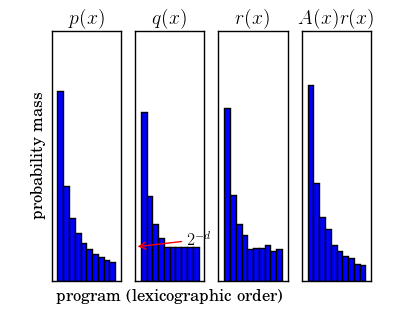
\includegraphics[width=8cm]{cartoon.png}
  \caption{\theSystem{} twice distorts the distribution $p(\cdot )$. First it introduces a parameter $d$ that bounds the tilt; we correct for this by accepting samples w.p. $A(x)$. Second it samples from $q(\cdot )$ by drawing instead from $r(\cdot )$, where $KL(q||r)$ can be made arbitrarily small by appropriately setting another parameter, $K$. $A(x)r(x)$ is distribution of samples.}\label{cartoon}
  \end{figure}

\subsection{Getting high-quality samples}
\textbf{Low-tilt approximation.}
We introduce a parameter into the sampling algorithm, $d$, that parameterizes $q(\cdot )$.
The parameter $d$ acts as a threshold, or cut-off, for the description length of a program;
the distribution $q(\cdot )$ acts as though any program with description length exceeding $d$ can be encoded using $d$ bits. Concretely,
\begin{equation}
  q(x) \propto \begin{cases}
    2^{-|x|},& \text{if } |x|\leq d\\
    2^{-d},              & \text{otherwise}
\end{cases}
  \end{equation}
If we could sample exactly from $q(\cdot )$, we could reject a sample $x$ with probability $1-A(x)$ where $A$ is
\begin{equation}
  A(x) \propto \begin{cases}
    1,& \text{if } |x|\leq d\\
    2^{-|x|+d},              & \text{otherwise}
    \end{cases}
  \end{equation}
and get exact samples from $p(\cdot )$, where the acceptance rate would approach 1 exponentially quickly in $d$.
\begin{proposition}\label{acceptanceBound}
  Let $x\in X$ be a sample from $q(\cdot )$. The probability of accepting $x$ is at least $\frac{1}{1 + |X|2^{|x_*|-d}}$ where $x_* = \argmin_x |x|$.
\end{proposition}
\begin{proof}
  The probability of acceptance is
  \begin{align}
    \sum_x q(x) A(x)& = \sum_x \frac{2^{-|x|}}{\sum_{x'}q(x')}\\
    & = \frac{Z}{Z + \sum_{|x| > d}(2^{-d} - 2^{-|x|}] }\\
      & > \frac{1}{1 + |X|2^{-d}/Z}>\frac{1}{1 + |X|2^{|x_*|-d}}.
  \end{align}
\end{proof}
%Two comments on Prop.~\ref{acceptanceBound}: (1) $Z$ is difficult to compute, and so we will use loose lower bounds; in fact $Z > 2^{-|x_*|}$ is sufficient for our later needs.
%A similar argument also shows that the KL between $p(\cdot )$ and $q(\cdot )$ is order $2^{-d}\frac{|X|}{Z}$.

The distribution $q(\cdot )$ is useful because we can guarantee that it has tilt bounded by
$d - |x_*|$.
Recent work has shown that the performance of nonuniform sampling via random projections degrades as the tilt increases~\cite{chakraborty2014distribution};
introducing the proposal $q(\cdot )$ effectively reifies the tilt,
making it a parameter of the program induction algorithm,
not the distribution over programs.

%as we show below:
We now show how to approximately sample from $q(\cdot )$ using a variant of the Embed and Project framework~\cite{ermon2013embed}.

\textbf{The embedding.} The idea is to define a new set of programs, which we call $E$, such that short programs are included in the set much more often than long programs.
Each program $x$ will be represented in $E$ by an amount proportional to $2^{-\min (|x|,d)}$, thus proportional to $q(x)$,
such that sampling elements uniformly from $E$  samples according to $q(\cdot )$.

We embed $X$ within the larger set $E$ by introducing $d$ \emph{auxiliary variables}, written $(y_1,\cdots, y_d)$,
such that every element of $E$ is a tuple of an element of $x = (x_1,\cdots , x_n )$ and an assignment to $y = (y_1,\cdots, y_d)$:
  \begin{equation}
    E = \{(x,y) \text{ }:\text{ } x\in X,  \bigwedge_{1\leq j \leq d} |x|\geq j\implies y_j=1 \}
  \end{equation}
  Suppose we sample $(x,y)$ uniformly from $E$.
  Then the probability of getting a particular $x\in X$ is proportional to
  \begin{align}
   & |\{(x',y)\in E \text{ : } x' = x\}| = \nonumber \\
    &| \{y\text{ : } |x|\geq j\implies y_j=1\}|=2^{\min (0,d-|x|)}
    \end{align}
  which is proportional to $q(x)$. Notice that $|E|$ grows exponentially with $d$, and thus with the tilt of the $q(\cdot )$. This is the crux of the inefficiency of sampling from high-tilt distributions in these frameworks:
  empirically, generating uniform samples using random projections, described below, becomes inefficient when the size of the support of the distribution is very high.

  \textbf{The random projections.} We  could sample exactly from $E$  by invoking the solver $|E|+1$ times to get every element of $E$,
  but in general it will have $O(|X|2^d)$ elements, which could be very large.
  Instead, we ask the solver for all the elements of $E$ consistent with $K$ random constraints
  such that (1) few elements of $E$ are likely to satisfy (``survive'') the constraints,
  and (2) any element of $E$ is approximately equally likely to satisfy the constraints.
  We can then sample a survivor uniformly to get an approximate sample from $E$, an idea introduced in the XORSample' algorithm~\cite{gomes2006near}.

  Our random constraints take the form of XOR, or parity constraints, which are random projections mod 2.
  Each constraint fixes the parity of a random subset of SAT variables in $x$ to either 1 or 0;
  thus any $x$ survives a constraint with probability $\frac{1}{2}$.
  A surprising feature of random parity constraints is that whether an assignment to the SAT variables survives is independent of whether another, different assignment survives.
  These events are even 3-wise independent, and these facts have been exploited to create a variety of approximate sampling algorithms~\cite{gomes2006near,valiant1985np,chakraborty2014balancing,gomes2006model}.
  
  Then the $K$ constraints are of the form $h\left(\begin{smallmatrix}x\\y\end{smallmatrix}\right) \modt b$ where $h$ is a $K\times (d+n)$ binary matrix and $b$ is a $K$-dimensional binary vector.
  If no solutions satisfy the $K$ constraints than the sampling attempt is rejected.

  These samples are close to uniform in the following sense: %, which strengthens the result in~\cite{gomes2006near}.
  \begin{proposition}\label{propositionLowerBound}
    The probability of sampling $(x,y)$ is at least $\frac{1}{|E|}\times \frac{1}{1 + 2^K/|E|}$ and the probability of getting any sample at all is at least $1 - 2^{K}/|E|$.
  \end{proposition}
  \begin{proof}
    The probability sampling $(x,y)$, given that $(x,y)$ survives the $K$ constraints,
    is $\frac{1}{\text{mc}}$, where $\text{mc}$ is the model count (\# of survivors).
    The probability of $(x,y)$ surviving the $K$ constraints is $2^{-K}$ and is independent of whether any other element of $E$ survives the constraints~\cite{gomes2006near}.
    So the probability of sampling $(x,y)$ is
    \begin{align}
      &      2^{-K}\sum_{i = 1}^{|E|} P(\text{mc} = i | (x,y) \text{ survives})\frac{1}{i}\\
      & = 2^{-K} E[\frac{1}{mc} | (x,y) \text{ survives} ] \\
      &> 2^{-K} \frac{1}{E[mc|(x,y) \text{ survives}]}\text{, Jensen's inequality}\\
      &= 2^{-K} \frac{1}{1 + (|E|-1)2^{-K}}\text{, pairwise independence}\\
      &> \frac{1}{|E|}\times \frac{1}{1 + 2^K/|E|}.
      \end{align}
    We fail to get a sample if $\text{mc} = 0$. We bound the probability of this event using Chebyshev's inequality: $E[\text{mc}] = |E|2^{-K}>\text{Var}(\text{mc})$, so
    \begin{align}
      P(\text{mc}= 0)&\leq P(|\text{mc}-E[\text{mc}]|\geq E[\text{mc}])\\
      &\leq \frac{\text{Var}(mc)}{E[\text{mc}]^2}<1/E[\text{mc}] = 2^K/|E|.
    \end{align}
  \end{proof}
  So we get approximate samples from $E$ as long as $|E|2^{-E}$ is not small.
  In reference to Fig.~\ref{cartoon},
  we call the distribution of these samples $r(x)=\sum_y r(x,y)$.
  Schemes more sophisticated than XORSample', like~\cite{ermon2013embed}, also guarantee upper bounds on sampling probability, but we found that these were unnecessary for our main result, which is that the KL between $p(\cdot )$ and $A(x)r(x)$ goes to zero exponentially quickly in a new quantity we call $\Delta$:
  \begin{proposition}\label{mainResult}
    Write $Ar(x)$ to mean the distribution  proportional to $A(x)r(x)$. Then $D(p||Ar)<\log \left( 1 + \frac{1 + 2^{ - \gamma}}{1 + 2^\Delta}\right)$ where
    $\Delta = \log |E| - K$ and $\gamma = d - \log |X| - |x_*|$.
  \end{proposition}
  \begin{proof}
      Define $c=\frac{1}{1 + 2^K/|E|}$. As $p(x)\propto A(x)q(x)$,
    \begin{align}
      D(p||Ar)& = \sum_x p(x)\log \frac{p(x)\sum_y A(y)r(y)}{A(x)r(x)}\\
      & = \sum_x p(x)\log \frac{A(x)q(x)}{\sum_y A(y)q(y)}\frac{\sum_y A(y)r(y)}{A(x)r(x)} \\ %\text{, as }q(x)A(x)\propto p(x)\\
      & = \log \frac{\sum_x A(x)r(x)}{\sum_x A(x)q(x)} + \sum_x p(x)\log \frac{q(x)}{r(x)}\\
      &  < \log \frac{\sum_x A(x)r(x)}{\sum_x A(x)q(x)} - \log c\label{lowerBound}
    \end{align}
    where~\ref{lowerBound} comes from Proposition~\ref{propositionLowerBound}.
    We know that $A(x)\leq 1 = A(x_*)$, that $r(x) \geq c q(x)$, and $\sum_x r(x) = P(\text{mc} > 0)$.
    Optimizing subject to these constraints,
    \begin{align}
      \sum_x A(x) r(x) &  < P(\text{mc} > 0) - \sum_{x\not= x_*} cq(x) +\sum_{x\not= x_*} cq(x)A(x)\nonumber\\
      & = P(\text{mc} > 0) + c \sum_{x} A(x) q(x) - c.
    \end{align}
    So the KL divergence is bounded above by
    \begin{align}
      D(p||Ar)&  < \log \left( c + \frac{P(\text{mc} > 0) -c }{\sum_x A(x)q(x)}\right) - \log c
    \end{align}
    The quantity $\sum_x A(x)q(x)$ is the probability of accepting a perfect sample from $q(\cdot )$,
    which Proposition~\ref{acceptanceBound} lower bounds:
    \begin{align}
      D(p||Ar)&  < \log \left( c + (1 -c)(1 + 2^{ - \gamma})\right) - \log c\\
      & = \log \left( \frac{1}{1 + 2^{ - \Delta}} + \frac{1 + 2^{ - \gamma}}{1 + 2^\Delta}\right)  + \log (1 + 2^{ - \Delta})
    \end{align}
    which for the sake of clarity we can weaken to% either
    \begin{align}
      D(p||Ar)&  < \log \left( 1 + \frac{1 + 2^{ - \gamma}}{1 + 2^\Delta}\right) . %< \frac{1}{\ln 2} \frac{1 + 2^{ - \gamma}}{1 + 2^\Delta}.
    \end{align}
  \end{proof}
  So we can approximate the true distribution $p(\cdot )$ arbitrarily well.
  Here we depart from the Unigen and Uniwit families of approaches~\cite{chakraborty2014distribution,chakraborty2014balancing} which only guarantee that the distribution of samples is with in a factor of 6.84 of the target distribution.
  Other approaches, like PAWS~\cite{ermon2013embed}, can prove analogously strong bounds.

  Application of Proposition~\ref{mainResult} requires knowledge $\min_x |x|$, which we compute using the iterative minimization routine in~\cite{singh2013automated}; in practice this is very efficient for finite program spaces. We also need to calculate $|X|$ and $|E|$, which are model counts that are in general difficult to compute exactly.
  However, many approximate model counting schemes exist, which provide upper and lower bounds that hold with arbitrarily high probability.
  We use Hybrid-MBound~\cite{gomes2006model} to upper bound $|X|$ and lower bound $|E|$ that each individually hold with probability at least $1-\delta / 2$ (see Alg.~\ref{mainAlgorithm}), thus
  giving lower bounds on both the $\gamma$ and $\Delta$ parameters of Proposition~\ref{mainResult} with probability at least $1-\delta$.
  and thus an upper bound on the KL divergence. 
 
  \begin{algorithm}[tb]
   \caption{\theSystem{}}
   \label{mainAlgorithm}
\begin{algorithmic}
  \STATE {\bfseries Input:} Program space $X$, failure probability $\delta$, natural numbers $\Delta$, $\gamma$,
  number of samples $N$
  \STATE {\bfseries Output:} $N$ samples 
  \STATE Set $|x_*| = \min_{x\in X} |x|$
  \STATE Set $B_X = $ ApproximateUpperBoundModelCount($X$,$\delta/2$)
  \STATE Set $d = \gamma + \log B_X + |x_* |$
  \STATE Define $E = \{(x,y) \text{ }:\text{ } x\in X,  \bigwedge_{1\leq j \leq d}  |x|\geq j\implies A_j=1 \}$
  \STATE Set $B_E = $ ApproximateLowerBoundModelCount($E$,$\delta/2$)
  \STATE Set $K = \log B_E - \Delta$
  \STATE Initialize samples $ = \varnothing$
  \REPEAT
  \STATE Sample $h$ uniformly from $\{0,1\}^{(d+n)\times K}$
  \STATE Sample $b$ uniformly from $\{0,1\}^{K}$
  \STATE Enumerate $S = \{ (x,y) \text{ where } h(x,y) = b \wedge x\in X\}$
  \IF{$|S| > 0$}
  \STATE Sample $(x,y)$ uniformly from $S$
  \IF{Uniform$(0,1) < 2^{d - |x|}$}
  \STATE samples $ = \text{samples}\cup \{x\}$
  \ENDIF
   \ENDIF
   \UNTIL{$|\text{samples}| = N$}
   \STATE {\bfseries return} samples
\end{algorithmic}
\end{algorithm}

  \textbf{Efficient enumeration.} The embedding $E$ introduces a symmetry into the solution space of the SAT formula, where one program (an $x$) corresponds to many points in the embedding (pairs $(x,y)$).
  We can more efficiently enumerate surviving members of $E$ by only enumerating unique surviving programs,
  and then counting the corresponding members of $E$ implicitly through the following result:
  \begin{proposition}\label{ranktheorem}
    Let $x\in X$ and $(x,y)\in E $ satisfy $h(a,y) \modt b$.  If $|x| \geq d$ then $(x,y)$ is the only surviving member of $E$ corresponding to $x$. Otherwise there are $2^{d - |x| - \text{rank}(g)}$ survivors where $g$ is the rightmost $d - |x|$ columns of $h$.
  \end{proposition}
  \begin{proof}
    If $|x|\geq d$ then there is only one element of $E$ corresponding to $x$.
    Otherwise,
    any assignment to $y$ satisfying
    \begin{equation}\label{eqmatrix}
      b \modt \left( \begin{array}{ccccc}
% &\vdots && \vdots& \\
h_{x} & \vdots& h_{y} &\vdots& g %\\
% & \vdots& & \vdots&
      \end{array} \right) \left( \begin{array}{c}
x \\
y_{\leq |x|} \\
y_{ > |x|}  \end{array} \right)
      %b_j  + \sum_{i = 1}^n h_{ji}x_i  + \sum_{i = n+1}^{n+|x|}h_{ji}A_{i - n}= \sum_{i = n + |x| + 1}^{n + d} h_{ji}A_{i - n}
    \end{equation}
    satisfies the random hashing constraints, where we have partitioned the columns of $h$ into those multiplied into $x$, $y_{\leq|x|}$, and $y_{ > |x|}$ .
    Because $(x,y)\in E$ the values of $x$ and $y_{\leq |x|}$ are fixed,
    so we can define a new vector $c \modt b + h_x x + h_y y_{\leq |x|}$ and rewrite Eq.~\ref{eqmatrix} as
    $c = g y_{ > |x|}$.
    Let $r = \text{rank}(g)$.
    Then there is a coordinate system where Eq.~\ref{eqmatrix} reads
    \begin{equation}\label{coordinateTransform}
      c \modt \left( \begin{array}{cccc}
        1&&&\\
        &\ddots&&\\
        &&0&\\
        &&&\ddots \end{array} \right) \left( \begin{array}{c}
        y_{1+|x|} \\
        \vdots\\
        y_{1+|x|+r}\\
        \vdots\end{array} \right)
    \end{equation}
    Eq.~\ref{coordinateTransform}     is satisfied iff, for all $1\leq j\leq r$, $y_{j+|x|} = c_j$.
    For $j > r$ the entries of $y_{j+|x|} $ are unconstrained,
    and so $2^{d  - |x| - r}$  satisfying values for $y$ exist.
  \end{proof}
  This enumeration strategy helps when sampling from sharply peaked posteriors,
  where there are few surviving programs; it also bounds the number of solver invocation to $|X|$.

  

  \subsection{Accuracy/Performance trade-off}
  We now analyze the runtime of Alg.~\ref{mainAlgorithm},
  using number of solver calls as a proxy for runtime.
  Our main results are that (1) the amortized time/sample decreases as we increase the dimension of the embedding,
  and (2) decreases as we increase the number of random constraints,
  which introduces a trade-off between accuracy of the samples and speed of the sampling.

  \begin{proposition}\label{proposition:tt}
    The expected number of calls to the solver per sample is bounded above by $\frac{1 + 2^\Delta}{(1 + 2^{ - \gamma})^{-1}(1 + 2^{ - \Delta})^{-1} - 2^{ - \Delta}}.$
  \end{proposition}
  \begin{proof}
    First upper bound the probability of failing, $P(\text{fail})$, to get a sample,
    which could happen if $S$  is empty or if the sample from $S$ is rejected,
    which is distributed according to $r(\cdot )$:
    \begin{align}
      P(\text{fail})& < P(\text{reject}) + P(\text{mc} = 0) \text{, union bound}\\
      & < 1 - \frac{\sum_x A(x)q(x)}{1 + 2^K/|E|} + 2^K/|E| \text{, Prop.~\ref{propositionLowerBound}}\\
      & < 1 - \frac{1}{(1 + 2^{ - \Delta})(1 + 2^{ - \gamma})} + 2^{ - \Delta}\text{, Prop.~\ref{acceptanceBound}}
    \end{align}
    The expected number of solver invocations per iteration is $< 1+E[\text{mc}] = 1 + |E|2^{-K} = 1 + 2^{\Delta}$
    and the expected number of iterations is $1/P(\neg\text{failure})$.
    Because the iterations are independent the expected number of solver invocations is just their product, which is the desired result.
  \end{proof}
  Proposition~\ref{proposition:tt} shows that the number of invocations to the solver grows exponentially in $\Delta$, while Proposition~\ref{mainResult} shows that the KL divergence from $p(\cdot )$ decays exponentially in $\Delta$.
  Algorithm~\ref{mainAlgorithm} balances this trade-off through its preliminary model counting steps; see Fig.~\ref{heat}.
  \begin{figure}
    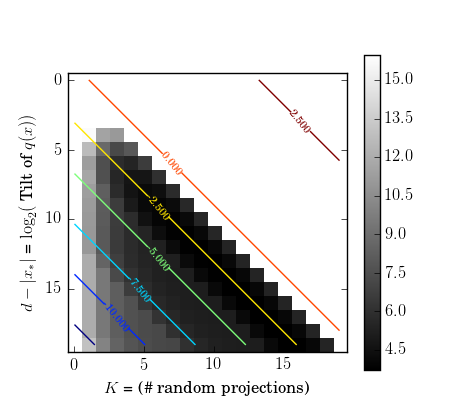
\includegraphics[width=7cm]{trade-off.png}
    \caption{Accuracy (colored contours) vs Performance (monochrome cells) trade-off for a program synthesis problem; upper bounds plotted. Performance measured in expected solver invocations; accuracy measured in log KL divergence. Prop.~\ref{acceptanceBound} lower bounds the tilt of performant samplers, while  Prop.~\ref{propositionLowerBound} upper bounds $K$ to $O(d)$, forcing our sampler into the darker (faster) regions.  KL divergence falls off exponentially fast in $\Delta = O(d - K)$, (Prop.~\ref{mainResult}) while solver invocations grows exponentially in $\Delta$ (Prop.~\ref{proposition:tt}) but is bounded by $|X|$ (Prop.~\ref{ranktheorem}), shown in white.}\label{heat}
    \end{figure}
     
  \section{Experimental results}

  We evaluated \theSystem{} on program learning problems in a text editing domain and a list manipulation domain.
  For each domain, we wrote down a sketch using the tool in~\cite{solar2006combinatorial}, specifying a large but finite set of possible programs.
  This implicitly defined a description-length prior, where $|x|$ is the number of bits required to specify $x$ in the SAT encoding.
We used   CryptoMiniSAT~\cite{crypto}, which can efficiently handle parity constraints.
  

\subsection{Learning Text Edit Scripts}
We applied our program sampling algorithm to a suite of programming by demonstration problems within a text editing domain.
Here, the challenge is to learn a small text editing program from very few examples
and apply that program to held out inputs.
This problem is timely, given the widespread use of the Flashfill program synthesis tool, which now ships by default in Microsoft Excel~\cite{real_world} and can learn sophisticated edit operations in real time from examples.
We modeled a subset of the Flashfill~\cite{Gulwani:2011:ASP:1926385.1926423} language;
our goal here is not to compete with Flashfill, which is heavily engineered for its specific domain,
but to study the behavior of our more general-purpose program learner in a real-world task.
To impart domain knowledge, we used a sketch equivalent to the following grammar:
\begin{verbatim}
Program ::= Term | Program + Term
Term    ::= String | substr(Pos,Pos)
Pos     ::= Number | pos(String,
                         String,Number)
Number  ::= 0 | 1 | 2 | ... 
         | -1 | -2 | ...
String  ::= Character 
         |  Character + String
Character ::= a | b | c | ...
\end{verbatim}
Because FlashFill's training set is not yet public, we drew text editing problems from~\cite{DBLP:conf/ecai/LinDETM14} and adapted them to our subset of FlashFill, giving 19 problems, each with 5 training examples.

We are interested both in the ability of the learner to generalize
and in \theSystem{}'s ability to generate samples quickly.
Tbl.~\ref{listTimes} shows the average time per sampling attempt using \theSystem{}, which is on the order of a minute.
These text edit problems come from distributions with extremely high tilt: often the smallest program is only tens of  bits long, but the program space contains (implausible) solutions with over 100 bits.
 By putting $d$ to $|x_*|-n$ we eliminate the tilt correction and recover a variant of the approaches in~\cite{ermon2013embed}. % (todo: is 2014 actually a variant of this?). chakraborty2014distribution
This baseline does not produce any samples for any of our text edit problems in under an hour.\footnote{Approximate model counting of $E$ was also intractable in this regime, so we used the lower bound $|E|\geq 2^{d-|x_*|} + |X| - 1$}

The learner generalizes to unseen examples, as Fig.~\ref{flashPerformance} shows.
We evaluated the performance of the learner on held out test examples as a function of training set size, and compares with baselines that either (1) enumerate programs in the arbitrary order provided by the underlying solver,
or (2) takes the most likely program under $p(x)$ (MDL learner).
The posterior is sharply peaked,
with most samples being from the MAP estimate,
and so our learner does about as well as the MDL learner.
However,
sampling offers an (approximate) predictive posterior over solutions to the held out examples;
in a real world scenario, one would offer the top $C$ solutions to the user
and let them choose,
much like how spelling correction works.
Performing this procedure allows us to offer the correct solutions more often than the MDL learner (Fig.~\ref{mdl}), because we are able to correctly handle ambiguous problems like in Fig.~\ref{ambiguous}.
\begin{figure}\centering
  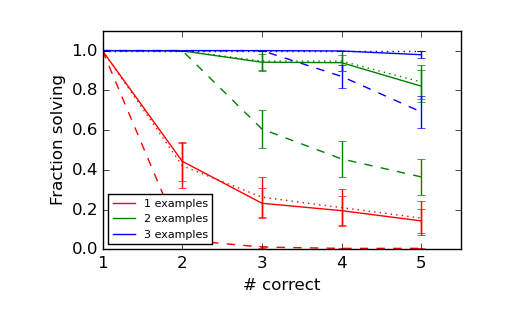
\includegraphics[width=0.4\textwidth]{fractionSolving.png}
  \caption{Generalization when learning text edit operations by example. Results averaged across 19 problems. Solid: 100 samples from \theSystem{} . Dashed: enumerating 100 programs. Dotted: MDL learner. Test cases past 1 (resp. 2,3) examples are held out when trained on 1 (resp. 2,3) examples.}\label{flashPerformance}
\end{figure}
 \begin{figure}
  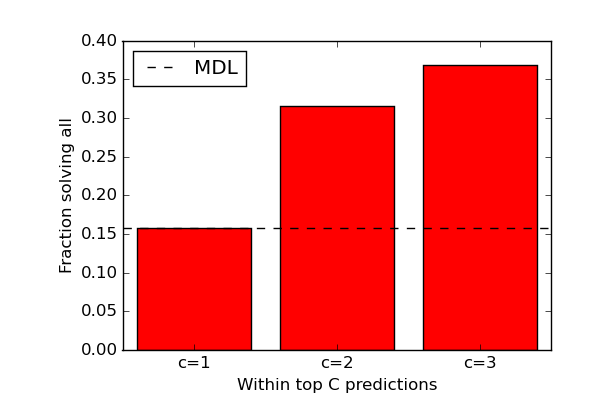
\includegraphics[width=0.5\textwidth]{mdl.png}
  \caption{Comparing the MDL learner (dashed black line) to program sampling when doing one-shot learning. We count a problem as ``solved'' if  the correct joint prediction to the test cases is in the top $C$ most frequent samples.}\label{mdl}
  \end{figure}

\begin{table}[]
\centering
\caption{Average solver time to generate a sample measured in seconds. See Fig.~\ref{listCurves} and \ref{flashPerformance} for training set sizes.}
\label{listTimes}
\begin{tabular}{l|lll}
  &      Large set      &  Medium set          &     Small set\\\hline
  text edit&49\pm 3 &21 \pm 1 &84 \pm 3 \\
sort    & 1549\pm 155 & 905 \pm 58   & 463 \pm 65  \\
reverse & 326\pm 42    & 141 \pm 18  &      39 \pm 3      \\
count        &    $\leq 1$          &   $\leq 1$          &          $\leq 1$
\end{tabular}
\end{table}  

\subsection{Learning list manipulation algorithms}
One goal of program synthesis is \emph{computer-aided programming}~\cite{solar2008program}, where a program induction system automatically generates executable code from either declarative specifications or examples of desired behavior.
Systems with this goal has been successfully applied to, for example, synthesizing intricate bitvector routines from specifications~\cite{gulwani2011automating}.
However, when learning from examples, there is often uncertainty over the correct program.
While past approaches have handled this uncertainty within an optimization framework (see~\cite{raychev2016learning,ellis2015unsupervised,singh2013automated}),
we show that \theSystem{} can \emph{sample} algorithms.
We take as our goal to learn recursive routines for sorting, reversing, and counting list elements from input/output examples,
particularly in the ambiguous,
unconstrained regime of few examples.

We wrote down a sketch with a set of basis primitives capable of representing a range of list manipulation routines equivalent to the following grammar:
\begin{Verbatim}[fontsize=\small]
Program   ::= (if Predicate List
                  (append RecursiveList
                          RecursiveList
                          RecursiveList))
Predicate ::= (<= Number) | (>= Number)
Number    ::= 0 | (1+ Number) | (1- Number)
            | (length List) | (head List)
List      ::= a | nil | (list Number)
            | (tail List)
            | (filter Predicate List)
RecursiveList ::= List | (recurse List)
\end{Verbatim}

A description-length prior that penalizes longer programs allowed learning of recursive list manipulation routines (from production \verb|Program|) and a non-recursive count routine (from production \verb|Number|); see Fig.~\ref{listCurves},
which shows average accuracy on held out test data when trained on variable numbers of short randomly generated lists.
With the large training set (5--11 examples) \theSystem{} recovers a correct implementation,
and with less data it recovers a distribution over programs
that functions effectively as a ``noisy algorithm''.

For some of these program learning tasks the number of consistent programs is small enough that we can enumerate all of them, allowing us to compare our sampler with the ground-truth probabilities.
Fig.~\ref{marginal} shows this comparison for a problem with 80 consistent programs, showing empirically that the tilt correction and random constraints do not significantly perturb the distribution.
\begin{figure}
  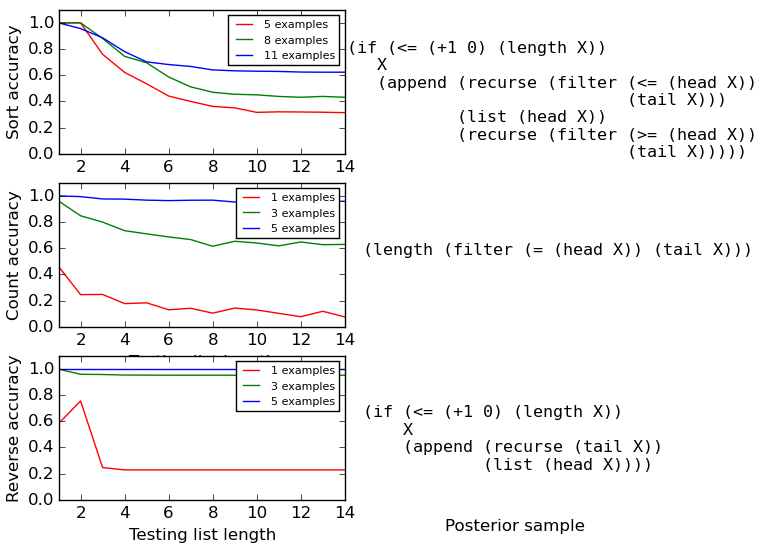
\includegraphics[width=0.5\textwidth]{list.png}
  \caption{Generalization performance of the program learner on list manipulation tasks. Trained on random lists of length $\leq 3$.}
  \label{listCurves}
\end{figure}
\begin{figure}
  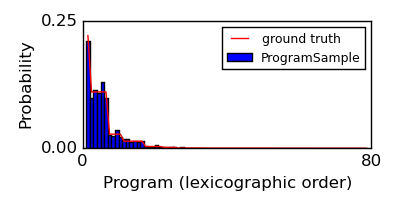
\includegraphics[width=0.4\textwidth]{probabilityPlot.png}
  \caption{Sampling frequency vs. ground truth probability for 1000 runs of \theSystem{} on a counting (see Fig.~\ref{listCurves}) task.}
  \label{marginal}
  \end{figure}

Tbl.~\ref{listTimes} shows the average solver time per sample; we see that generating recursive routines like sorting and reversing is much more costly than generating the nonrecursive counting routine.
Our constraint-based approach propositionalizes higher-order constructs like recursion, and so reasoning about them is much more costly.




\section{Discussion}

\subsection{Related work}
There is a vast literature on program learning within the AI and machine learning communities.
Many employ a (possibly stochastic) heuristic search over structures using genetic programming~\cite{DBLP:books/daglib/0070933} or MCMC~\cite{schkufza2013stochastic}.
These approaches often find good programs and can discover more high-level structure than our approach.
However, they are prone to getting trapped in local minima
and, when used as a sampler, determining the mixing time is in general not possible.
Recently researchers have turned to the problem of learning good priors over programs in a multitask setting~\cite{DBLP:conf/icml/LiangJK10,menon2013machine,Dechter:2013:BLV:2540128.2540316}.
We see our work here as particularly complementary to these methods: while they focus on learning the structure of the hypothesis space,
we focus on efficiently sampling an already given hypothesis space (the sketch).
There are several recent proposals for recurrent deep networks that learn algorithms~\cite{DBLP:journals/corr/ReedF15,graves2014neural}.
We see our system working in a different regime,
where we want to quickly learn an algorithm from a small number of examples or an ambiguous specification.

The program synthesis community has several recently proposed learners that work in an optimization framework~\cite{raychev2016learning,ellis2015unsupervised,singh2013automated}, and these motivate our description length prior.
By computing a posterior over programs, we can more effectively represent uncertainty, particularly in the small data limit, but at the cost of more computation: our algorithm requires an optimization routine to calibrate the sampler.


Our sampling algorithm borrows heavily from a line of work started in~\cite{gomes2006near,gomes2006model} on sampling of combinatorial spaces using random XOR constraints, which is motivated by results in complexity theory~\cite{valiant1985np}.

\subsection{Limitations of the approach}

The constraint-based synthesis methods on which our technique is built tend to excel in domains where the structure of the expected solutions can be restricted by a ``sketch''~\cite{solar2008program} and where much of the program's description length can be easily computed from the program text. 
For example, \theSystem{} can synthesize text editing programs taking almost 60 bits of description length in a couple seconds, but spends 10 minutes synthesizing a recursive sorting routine that takes fewer bits of description length but where the program structure is less restricted. 
Constraint-based methods also require the entire problem to be represented symbolically, so they have trouble when the function to be synthesized involves complex building blocks such as numerical routines that are difficult to analyze.
For such problems, methods based on stochastic search~\cite{nori2015efficient,schkufza2013stochastic,DBLP:books/daglib/0070933} can be more effective because they only need to be able to run the functions under consideration. Finally, past work has also shown empirically that constraint-based approaches scale poorly with data set size, although this can be mitigated with clever approaches to consider data incrementally ~\cite{ellis2015unsupervised,raychev2016learning}.


The requirement of producing representative samples imposes some additional overheads on our approach, so scalability can  more limited than for standard symbolic techniques on some problems. For example, our method requires 1 MAP inference query, and 2 queries to an approximate model counter for every new problem. The approximate model counter serves to ``calibrate'' the sampler, and its cost can be amortized because it only has to be invoked twice in order to generate an arbitrary number of iid samples. Approximate model counters like MBound~\cite{gomes2006model}
have complexity comparable with that of generating a sample, but the complexity is strongly dependent on the number of solutions to the system. 
Thus, for good performance, \theSystem{} requires that there not be too many programs consistent with the data---the largest spaces considered in our experiments had  $\leq 10^7$ programs. This limitation, together with the general performance characteristics of symbolic techniques, means that the approach will work best for ``needle in a haystack'' problems, where the space of possible programs is large but restricted in its structure, and where only a small fraction of those programs satisfy the semantics constraints.


\subsection{Future work}
This work could naturally extend to other domains that involve inducing latent symbolic structure from small amounts of data,
such as semantic parsing to logical forms~\cite{liang11dcs},
synthesizing motor programs~\cite{lake2015human},
or learning relational theories~\cite{logical}.
These applications have some component of transfer learning,
and building efficient program learners that can transfer inductive biases across tasks is a prime target for future research.
\pagebreak
\bibliography{main}
\bibliographystyle{icml2016}

\end{document} 


% This document was modified from the file originally made available by
% Pat Langley and Andrea Danyluk for ICML-2K. This version was
% created by Lise Getoor and Tobias Scheffer, it was slightly modified  
% from the 2010 version by Thorsten Joachims & Johannes Fuernkranz, 
% slightly modified from the 2009 version by Kiri Wagstaff and 
% Sam Roweis's 2008 version, which is slightly modified from 
% Prasad Tadepalli's 2007 version which is a lightly 
% changed version of the previous year's version by Andrew Moore, 
% which was in turn edited from those of Kristian Kersting and 
% Codrina Lauth. Alex Smola contributed to the algorithmic style files.  
